\documentclass[a4paper,10pt]{scrartcl}
\usepackage[utf8]{inputenc}

\usepackage{amsmath}
\usepackage{amsfonts}
\usepackage[english]{babel}
\usepackage{fontenc}

% Added packages
\usepackage{graphicx}
\usepackage{xcolor}
\usepackage{booktabs}

% CUSTOM COMMANDS
\newcommand\todo[1]{\textcolor{red}{TODO: #1}}
\newcommand\TODO[1]{\textcolor{red}{TODO: #1}}
\newcommand\eve{\textit{Eve}}
\newcommand\alice{\textit{Alice}}


% Title Page
\title{Digital Forensics - Project Report}
\subtitle{Project 1 - Packet classification for mobile applications}
\author{Eugen Saraci - 1171697\\ Università degli Studi di Padova \\\texttt{\small{eugen.saraci@studenti.unipd.it}}}

\begin{document}

\maketitle
\begin{abstract}
The large expansion of SSL/TLS has made it harder for attackers to collect clear text information through packet sniffing or, more in general, through network traffic analysis. The main reason for this is that SSL/TLS encrypts the traffic between two endpoints, which means that even though packets can still be easily captured, no useful information can be inferred from the packets' content without having the encryption keys.\footnote{It is worth mentioning that the endpoints of the communication (i.e. source and destination IP addresses) are transmitted in clear text for routing purposes; by performing a DNS lookup of the addresses and attacker could easily infer what site a user is visiting.}

The authors of \cite{contiknocking} and \cite{contianalysis} showed that by training a machine learning algorithm with encrypted traffic data, one could correctly classify which actions a user performed while using some of the most common Android applications such as Facebook, Gmail, or Twitter. This could easily lead, through correlation attacks, to the full deanonimization of fake, privacy preserving identities.

In this work I try to replicate the results achieved in \cite{contiknocking} and \cite{contianalysis} by implementing the classification model as described in the papers.
\vspace{0.5cm}
\end{abstract}

\section{Introduction and Notation}
\label{sec:intro}

\subsection{Actions and Flows}
\label{subsec:flows}
In order to easily understand this work, in the next two subsections I introduce two general concept used throughout this report.

\subsubsection{Action and Action Label}
An \textit{action} is simply the action performed by a user while using one of the aforementioned Android apps. Examples of actions are: clicking on a profile page, tweeting a message, sending an email etc. Please note that ``clicking on a profile page'' is what I refer to as the \textit{action label}, in many cases I use the words ``action'' or ``action flow'' to refer to the set of flows that represent that action.

\subsubsection{Flows}
When a user performs an action some encrypted packets are exchanged with the destination server. A flow consists of the sequence of the byte sizes of the exchanged packets. If the packet is going from the user's phone to the server it is said to be \textit{outgoing}; if the packet is coming from the server to the user's phone it is said to be \textit{incoming} and it is marked with a ``-'' sign before the integer number representing its size.\footnote{The ``-'' sign is just notation, packets cannot have a negative size.} An example of a 5 packet flow is: \texttt{[-12, 80, 90, -111, 30]}. Please note that a single action performed by the user usually generates multiple flows of different dimensions, by that follows that an action actually consists of multiple flows. The techniques used by the authors to determine which flows belong to which action, the ordering of the packets, the packet capturing system, the packet filtering system, and the statistical analysis on the flows will not be treated in this report since the starting point for this work comes when the dataset is already constructed.

\subsection{Notation}
\label{subsec:notation}
\begin{itemize}
 \item $ A $: an action; it represents a sequence of flows;
 \item $ a $: action label;
 \item $ F $: a flow; it represents a sequence of packets;
 \item $ p $: a single packet, it is an integer number representing the size in bytes of that packet.
\end{itemize}

Please note that all of the above can be subscripted by indexes; a subscripted element means that that element is the i-th element of a sequence, e.g. $F_i$ is the $i$-th flow of a sequence of flows (possibly an action $A$).
 
By this follows that $A_i = [F_1, \dots, F_n]_i$ and $F_i = [p_1,\dots, p_m]_i$. Note that $n$ and $m$ are possibly (and probably) different for each flow $F_i$ and for each action $A_i$, even for two actions $A_i, A_j$ where $a_i = a_j$.

\subsection{Dataset}
The dataset consists of 252,151 rows (samples) and 12 columns (features), moreover, the data collected contains packets of different actions for 7 different Android applications: Facebook, Twitter, Gmail, Google Plus, Tumblr\footnote{Because of some inconsistencies between the papers and the dataset, I could not provide a classifier for the Tumblr's actions.}, Dropbox, and Evernote. 

In Table \ref{tab:origdataset} we can see the format of the dataset. I have purposively hidden some of the columns since I do not use them in this work. In the table we can see that each row contains the features of a single flow; to decide which flows belong to which action we compare the \textit{sequence\_start} field which is a fake but consistent timestamp of when the user started that action; When two rows have the same timestamp we can safely assume that they belong to the same action.


\begin{table}[]
\label{tab:origdataset}
\begin{tabular}{@{}lllll@{}}
\toprule
\textbf{action\_start}      & \textbf{app}               & \textbf{action\_label}     & \textbf{\dots}             & \textbf{flow}                \\ \midrule
1383129102.11              & facebook                   & open facebook              & \dots                      & [-15, 75, 144]               \\
1383129102.11              & facebook                   & open facebook              & \dots                      & [-55, -255, -333, 122, -55]  \\
\multicolumn{1}{c}{\dots} & \multicolumn{1}{c}{\dots} & \multicolumn{1}{c}{\dots} & \multicolumn{1}{c}{\dots} & \multicolumn{1}{c}{\dots}   \\
1383129102.11              & facebook                   & open facebook              & \dots                      & [12, 12, 155, 155, -18, 255] \\
1383129244.01              & facebook                   & click menu                 & \dots                      & [78, -206]                   \\
\multicolumn{1}{c}{\dots} & \multicolumn{1}{c}{\dots} & \multicolumn{1}{c}{\dots} & \multicolumn{1}{c}{\dots} & \multicolumn{1}{c}{\dots}   \\ \bottomrule
\end{tabular}
\caption{\small{Some rows of the dataset.}}
\end{table}

\section{Machine Learning}
\label{sec:ml}

\textbf{Goal}: as in Figure~\ref{fig:ideal} we want a machine learning algorithm $\mathcal{L}$ that predicts the \textit{action label} $a_i$ given the \textit{action's flows} $A_i = [F_1,\dots, F_n]_i$.

\begin{figure}[h]
 \centering
 
\includegraphics{images/ideal}
 \caption{\small{The ideal model predicting the label $a_i$ for the a new input instance $A_i$.}}
 \label{fig:ideal}
\end{figure}

Given the fact that each action generates multiple flows of different lengths, we know that standard supervised learning approaches are hard to apply. To see why standard approaches would not work we need to think about the structure of the input and output spaces. Our output space i.e. what we want to predict would be the \textit{action label} $a_i$, while our input space, i.e. the predictors, would be the flows generated by $a_i$ which we denote as $[F_1,\dots,F_n]_i $. One way we could represent flows as features would be to have a feature for each flow $F_j$ generated by the action $a_i$, and the value of the $j$-th feature would be the sequence of byte sizes of the flow $[p_1,\dots, p_m]_j$. Because of the different number of flows for each action  $n$ we would immediately see that each row could possibly have a different number of features. The main issue with this approach, however, other than the just mentioned diverse dimensionality, is that we are artificially defining features with no real justification; in other words, we have no reason to associate the first flow of an action $A_i$ with the first flow of another action $A_j$ by interpreting them as the first feature of their respective samples.


To overcome this obstacle, the original authors applied a two stage process: in the first stage the objective is to identify, thanks to an unsupervised clustering algorithm, some kind of intermediate representation of the data $\Phi(A_i)$; in the second stage the aim is to use that intermediate representation to perform a canonical classification task (Figure~\ref{fig:actual}). 
In the remainder of this section we describe the algorithms used in the two stage process while my personal implementation is presented in Section \ref{sec:eval}.

\begin{figure}[h]
 \centering
 
\includegraphics{images/actual}
 \caption{\small{The two step classification of a new sample; first the new sample $A_i$ goes through the clustering algorithm which computes the intermediate representation $\Phi(A_i)$, then $\Phi(A_i)$ is used by the classifier to predict the correct label $a_i$. $k$ is the number of clusters, a more detailed description of $k$ and $\Phi$ can be found in subsections~\ref{subsubsec:hac} and \ref{subsubsec:fexc}.}}
 \label{fig:actual}
\end{figure}

\subsection{Clustering}
In the typical unsupervised clustering scenario the goal of the algorithm is to find $k$ groups called clusters, where the \textit{inter-cluster} similarity is very low while the \textit{intra-cluster} similarity is maximized, meaning that samples belonging to one clusters are very similar to each other while still being very different from samples belonging to other clusters. Notice that the number of clusters $k$ and the similarity function between samples have to be explicitly defined by the teacher and both have a significant impact on the final result. The input of the clustering algorithm is usually the whole dataset while its output is a list of integers $[c_1,\dots, c_N]$ where $N$ is the total number of samples and $c_i \in [1;k]$ is a an integer number that denotes the cluster to which the $i$-th sample has been assigned by the algorithm.

\subsubsection{Hierarchical Agglomerative Clustering}
\label{subsubsec:hac}
In this specific instance I used (as suggested in the papers) a \textbf{Hierachical Agglomerative Clustering}, \textbf{HAC} for short. HAC starts by creating a cluster for each flow; at each step HAC reduces the number of clusters by merging (agglomerative) the closest clusters together based on the distance function and other parameters; HAC will stop whenever the desired number of clusters $k$ is reached. The structure that HAC exploits can be seen as a tree (hierachical), that structure is called dendrogram; in Figure \ref{fig:dendro} we can see the dendrogram for 20 samples (i.e. 20 flows). In my implementation the input consists of all the flows contained in the dataset\footnote{We are just using flows now, the concept of ``actions'' is being ignored for the moment since it is not really needed for the clustering stage.}, the number of clusters $k$ is set to $250$, and the distance function used to compute similarity between flows is Dynamic Time Warping.

\begin{figure}[!h]
 \centering
 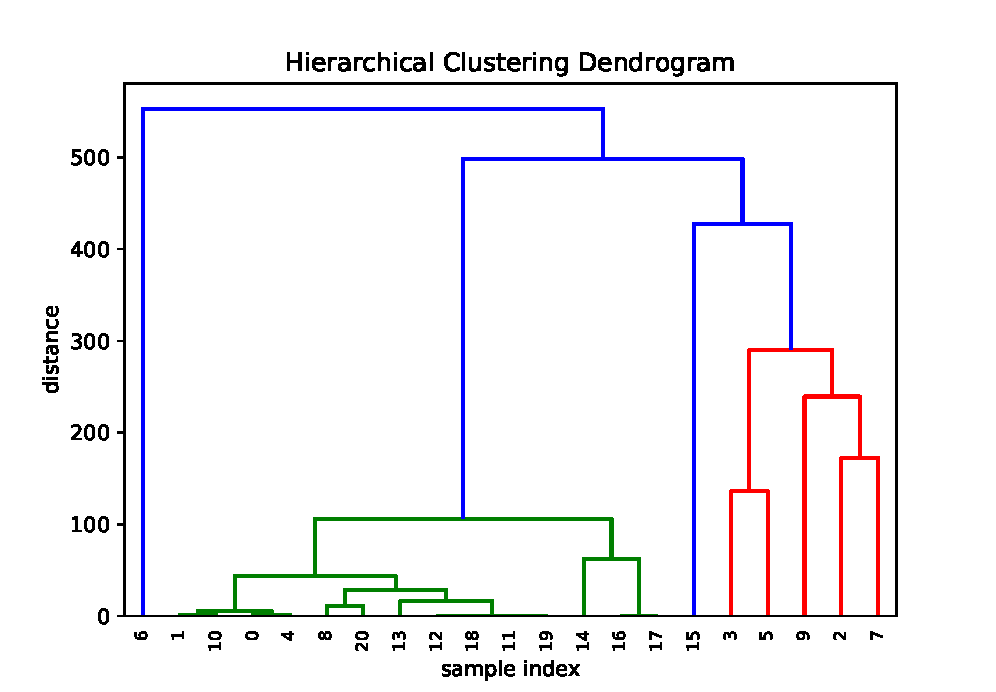
\includegraphics[scale=0.5]{images/dendrogram}
 \caption{\small{Dendrogram for 20 flows; the number of clusters can be seen by counting how many vertical lines get crossed by an imaginary horizontal line. Different horizontal lines will of course determine different clusters and different distance measures; the dendrogram allows the designer to decide at what level to draw the line i.e. which value to assign to $k$ by looking at the distance value and at the hierarchy itself.}}
 \label{fig:dendro}
\end{figure}

\subsubsection{Dynamic Time Warping}
\label{subsubsec:dtw}
\textbf{Dynamic Time Warping} or \textbf{DTW} is an algorithm generally used to find the best match between two time series even when they have different lengths and/or have repetitions or deletions in them. If we view every single flow $F_i$ as a series of packets $[p_1,\dots p_m]_i$, we can use DTW to measure how similar two flows are. This similarity measure is needed by the HAC algorithm to compute the distances between clusters.

\subsubsection{Feature Extraction}
\label{subsubsec:fexc}
The HAC output is, as stated before, a list of $N$ integers $[c_1,\dots, c_N]$ where $c_i$ is the cluster assigned to the $i$-th input sample. This is different from what is reported in Figure \ref{fig:ideal}, in fact the clustering result needs to be rearranged before being given as input to the classifier. The aim of the rearrangement is to actually generate a new intermediate dataset where the targets we want to predict are still the actions' labels, but the features are now different. We generate $k$ features for each action $A_i$; the value of the $j$-th feature is the number of flows of $A_i$ that ended up in the $j$-th cluster during the clustering algorithm. This whole process, composed by the \textit{clustering} and the final rearrangement, is what we call feature extraction and we denote it with the symbol $\Phi$, so $\Phi(A_i)$ is the intermediate representation of a sample $A_i$ and it is considered to be a single input instance of the new intermediate dataset.

\begin{table}[]
\label{tab:newdataset}
\centering
\begin{tabular}{@{}lcccc@{}}
\toprule
\textbf{action\_label}     & \multicolumn{1}{l}{\textbf{C1}} & \multicolumn{1}{l}{\textbf{C2}} & \multicolumn{1}{l}{\textbf{\dots}} & \multicolumn{1}{l}{\textbf{C250}} \\ \midrule
open facebook              & 0                               & 11                              & \dots                              & 6                                \\
writing search             & 1                               & 1                               & \dots                              & 5                                \\
back to news               & 0                               & 0                               & \dots                              & 0                                \\
open facebook              & 0                               & 9                               & \dots                              & 5                                \\
\multicolumn{1}{c}{\dots} & \dots                          &                                 & \dots                             & \dots                           \\ \bottomrule
\end{tabular}
\caption{\small{Format of the new dataset. We can see that 11 flows of the first action ended up in cluster number 2, while 6 of them ended up in the last cluster.}}
\end{table}

\subsection{Classification}
Now that we have a suitable dataset we can apply a supervised classification machine learning algorithm. In this scenario we split the data in two disjunct sets: \textit{training} and \textit{test set}; the first will be used to train the classifier while the other will test if the algorithm actually learned the concept that correlates the intermediate representation $\Phi(A_i)$ to the label $a_i$. The machine learning algorithm chosen is \textbf{Random Forest}.

\subsubsection{Random Forest Classifier}
\label{subsubsec:rfc}
The Random Forest Classifier is, as the name says, a classifier; its two main features can also be explained by analyzing its name:
\begin{itemize}
 \item \textbf{Forest}: it is a collection of decision trees (which are (\textit{weak}) classifiers themselves); if we want to classify a new instance on an already trained forest, what happens under the hood is that the forest will pass that instance to all of its trees and each one of them will return a prediction for that instance; the output of the forest will be the prediction voted the most by its trees.\footnote{Some variants will weight the vote of each tree differently based on their performances.}
 \item \textbf{Random}: in Random Forest there are two degrees of randomness; during training phase each tree has to be built using:
 \begin{itemize}
  \item a random subset of the total input data;
  \item a random subset of features extracted from all the features available (usually $\sqrt{\text{total number of features}}$).
 \end{itemize}
\end{itemize}

To better understand how Random Forest works it is worth mentioning the basic structuture and mechanisms we find in Decision Trees. 

\paragraph{Structure of Decision Trees}
\begin{itemize}
 \item \textbf{nodes}: each internal node (root node included) can be represented by the subset of the samples it is working with (the root node is working with the whole dataset) and by the decision that has to be made at that node; the decision is just a boolean expression that gets applied to the all elements of the current subset. 
 \item \textbf{arcs}: the arcs are the possible outcomes of the decision at a given node; the elements of the subset of the node will be sent down the arc they ``satisfy''.
 \item \textbf{leaf nodes}: leaf nodes are predictions (this means they are possible values of $a$ or \textit{action labels}), a leaf node is formed when all the elements of a given node have the same class/target/$a$/\textit{action label}.
\end{itemize}

\paragraph{Mechanisms of Decision Trees}
The aim of the Decision Tree is to generate at each node the purest possible subsets, to do so it uses (im)purity measures (Information Gain) or dispersion measures (Gini Index). At each node only one feature is tested, the outgoing arcs of a node are the number of possible values that the feature can assume (if discrete) or a threshold value (if real), in which case only two arcs will be generated. Both the feature and the threshold (if any) are chosen based on the criteria cited previously. In addition to what has been said in the previous paragraph: a leaf node can be formed also when there are no more features to test (they have all been tested in previous nodes), in this case the prediction of the leaf node will be the \textit{action label} with higher frequency on that subset. A small part of a Decision Tree can be seen in Figure \ref{fig:tree}, the colors and their intensity are used to highlight which \textit{action label} is more frequent at each node.

\begin{figure}[!h]
 \centering
 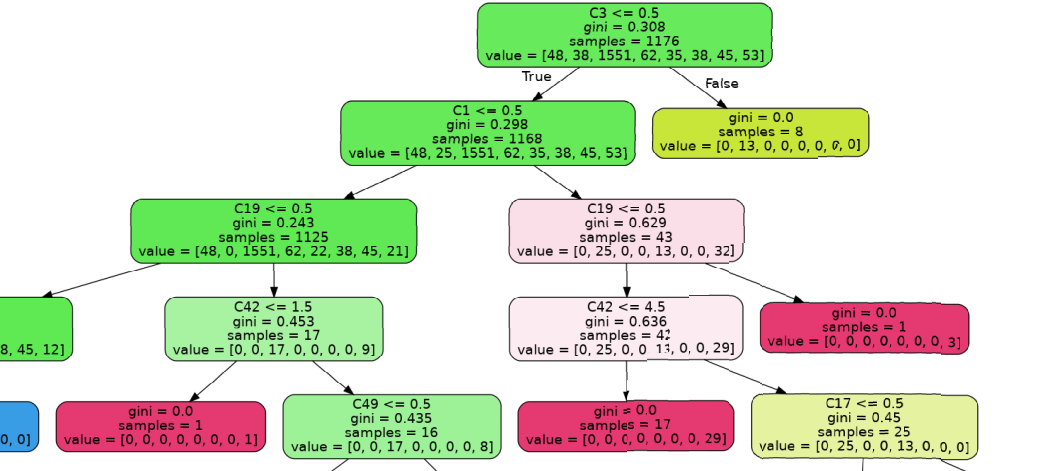
\includegraphics[scale=0.4]{images/tree}
 \caption{\small{Small part of a single tree of the forest. At each node the value of a given feature is tested, the arcs opening to the left satisfy the condition while those to the right do not. In my implementation the number of trees in the forest is 10.}}
 \label{fig:tree}
\end{figure}



\section{Evaluation}
\subsection{Experimental Setup}
For this work I implemented two scripts using Python 3.6.5. The two scripts represent the two stages of clustering and classification shwon in Figure~\ref{fig:actual}; the first script, named \texttt{clustering.py}, performs the clustering and saves the intermediate representation as a .csv file called \texttt{[appname]\_dataset.csv}. This file is read as input by \texttt{classifier.py} which will consequently perform the classification using the Random Forest algorithm presented in Section~\ref{subsubsec:rfc}. The computed performance measures will be printed to \texttt{stdout}.

\subsubsection{Computational Issue}
Because of some issues with the functions provided by the Python library \texttt{scipy} I had keep in memory the distance matrix of the flows. In the distance matrix $D$ every entry $(i,j)$ is the vlaue of $dtw(i, j)$ which makes $D$ symmetric, which reduces by half the memory needed for the matrix since I could just compute the tringular upper (or lower) part of $D$. Unfortunately this ``optimization'' was not enough, the

\todo{dire che non usiamo il dataset totale e motivare, dire gcloud, dire computational issues with dtw nello specifico, qui cito i praametri/input/output di entrambi gli algoritmi}
\todo{spiegare le azioni tagliate fuori}
\subsection{Experimental Results}
\todo{le confusion matrix, precision recall AP}

%  \section{Final Notes}
 In conclusion, the aim of this work was to replicate what has been done in \cite{contiknocking} and \cite{contianalysis}; due to time and computational limitations I had to simplify my model, and luckily no loss of performance was encountered, allowing me to successfully reach the original results. Since the original papers might be a little outdated (the traffic data was captured in 2014), it might be interesting to perform the same kind of attack using current day's network traffic and evaluate if such issues still persist.
 
All the scripts, the datasets, the confusion matrixes, can be found at: https://github.com/esaraci/knocking.


\begin{thebibliography}{99}
\bibitem{contiknocking} Mauro Conti, Luigi V. Mancini, Riccardo Spolaor, and Nino Vincenzo Verde. 2015. Can't You Hear Me Knocking: Identification of User Actions on Android Apps via Traffic Analysis. In Proceedings of the 5th ACM Conference on Data and Application Security and Privacy (CODASPY '15). ACM, New York, NY, USA, 297-304. DOI: https://doi.org/10.1145/2699026.2699119
\bibitem{contianalysis} Conti, M., Mancini, L. V., Spolaor, R., \& Verde, N. V. (2016). Analyzing android encrypted network traffic to identify user actions. IEEE Transactions on Information Forensics and Security, 11(1), 114-125.

\end{thebibliography}

\end{document}
